\section{Hybrid Criticality Scheduler}
\label{sec.scheduling.hybrid}

The Hybrid Criticality Scheduler (HYBRID) is a combination of the CATS and CPATH scheduling policies.
HYBRID keeps the simplicity of the implementation of CATS and introduces the task execution time only if available.
This results in an efficient low-overhead scheduler that computes the critical path of a TDG more faithfully than CATS and with lower overheads than CPATH.
%The idea for this is again based on separating the critical and non-critical tasks and execute the critical tasks on the fast cores of the system.
This section describes HYBRID through its relation to CATS and CPATH described in Sections~\ref{sec.scheduling.cats} and~\ref{sec.scheduling.cpath}. 
We focus our description on the task prioritization, since task submission and task-to-core assignment for HYBRID are identical to CPATH.

As shown, CPATH computes priorities on task completion. 
The algorithm for priority computation is an expensive operation and is in the critical path of the execution:
on task completion the core becomes available but the start of the next task is delayed by priority computation.
Also, when multiple cores are completing tasks, there will be contention on accessing the TDG for priority computation.
On the other hand, CATS computes priorities during task creation.
The computation of priorities during task creation is more efficient because, unless there is nested parallelism, one core creates all tasks and therefore there is no contention due to multi-threading on priority computation. 
The downside is that there is potentially less information available on tt-is pair execution time on task creation, as some task type may have not been executed yet at the time all tasks are created.
%there is only one core involved in this procedure responsible for the creation of the tasks.
%In addition, the rest of the cores are exclusively used for executing tasks undisturbed.

%, where it is more unlikely to have information about the task execution time. 

%In an effort to reduce the scheduling overheads of CPATH, we implement HYBRID. 
HYBRID tracks task execution time on task completion and stores this information in a vector.
This means that it also implements the \texttt{taskExit} function of CPATH that is called on task completion but, in the case of HYBRID, \texttt{taskExit} is only responsible of recording the execution time of the exiting task.
This functionality is represented in lines 2-9 of Listing~\ref{cpathExit} and, after this code, the function returns.
% in HYBRID takes place during task creation because as described above this reduces the scheduling overheads.
The priority assignment, taking place on task creation, remains similar to CATS \footnote{All of the HYBRID scheduling steps have the same time complexity as CATS} with the only difference that task cost is used for priority computation only if known and, otherwise, the cost is assigned to 1 and priority is increased according to CATS (lines 7 and 8 of Listing~\ref{creation}).

%high-level differences:
%% This could be simplified, also given there is a short mention before
When comparing CPATH and HYBRID schedulers their logical operation is similar.
However the difference in their implementation may result in different task priorities potentially leading to different schedules.
For applications with small TDGs, HYBRID may not be able to compute an accurate critical path because task creation does not overlap with a sufficient amount of task exits.
%Therefore, priority computation will not have enough information about task execution time and HYBRID will prioritize based on bottom-level priorities (like CATS).
Therefore, task execution information will not be available during priority computation and HYBRID will prioritize based on bottom-level priorities (like CATS).
If the application has a large TDG and task creation overlaps with a sufficient amount of task exits, HYBRID will use bottom-cost priorities.
%CPATH on the other hand, updates priorities right after task cost is known, which leads to a more faithful critical path computation. 

\begin{figure}[t]
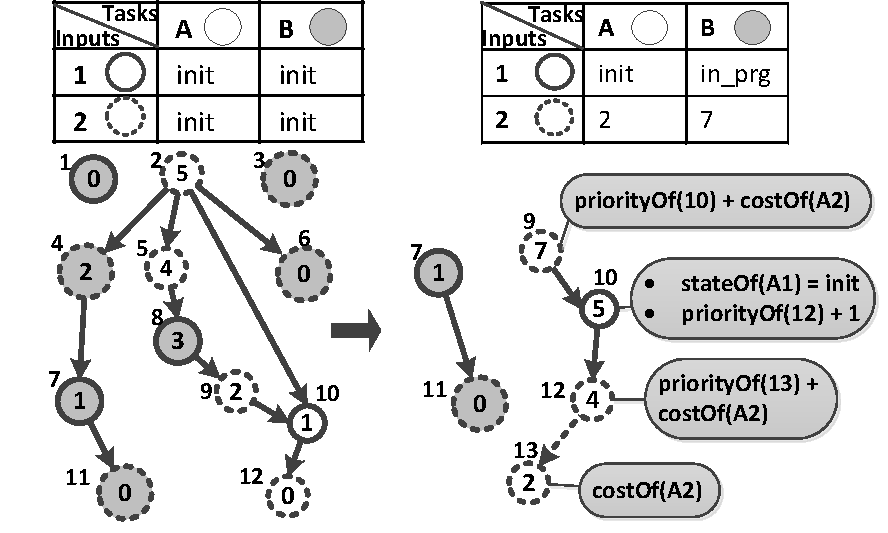
\includegraphics[width=\columnwidth]{images/hybrid_prioritization.pdf} 
\centering
\caption{Priority assignment with HYBRID scheduler. Priority update when the edge between tasks 12 and 13 is created}
\label{hybrid_priorities}
\vspace{-0.5cm}
\end{figure} 

Figure~\ref{hybrid_priorities} shows an example of task prioritization with HYBRID.
The tables show the state (or exec. time) of the tt-is pairs that appear on the TDG. Gray or white nodes indicate different task types (A or B respectively) and solid or dashed node outlines indicate task input size (1 or 2 respectively). The numbers inside the nodes show task priorities and the numbers outside the nodes show the task id.

On the leftmost TDG, the algorithm has no information about any of the tt-is costs.
As the leftmost table shows, for all the possible tt-is the state is \texttt{init} meaning no task has been executed yet.
Since the tasks of the TDG have been created, they have been prioritized using the CATS priority assignment method and the bottom level based priorities.
On the rightmost TDG, tasks 1, 2, 3, 4, 5, 6 and 8 have been executed and a new task has appeared on the TDG: task number 13.
When the edge 12$\rightarrow$13 is created, tasks begin to be prioritized.
Initially, the priority of the new task 13 is the cost of this task's tt-is, i.e., type A and input 2 (TaskA-Input2). 
Since there are no successors of this task, this becomes its initial priority.
Then, the \textit{plist} of task 13 is traversed and the priority of task 12 changes to priorityOf(13)+costOf(TaskA-Input2) since task 12 is corresponding to the TaskA-Input2 tt-is.
Moving to the upper levels, task 10 is of tt-is TaskA-Input1 that is on the \texttt{init} state, thus unknown cost.
This translates to the use of bottom level based prioritization so the priority of task 10 becomes priorityOf(12)+1.
Finally, task 9 is prioritized using the cost of the TaskA-Input2 tt-is and the TDG navigation stops since there are no other predecessors.

\if 0


Like CPATH, HYBRID prioritizes tasks according to their \textit{bottom cost} and/or their \textit{bottom level}.

HYBRID constitutes of three steps: \textit{Task Prioritization, Task Submission} and \textit{Task-to-core assignment.}


\subsection{Task prioritization}
The HYBRID scheduler prioritizes tasks according to their \textit{bottom cost} and/or their \textit{bottom level}.
The task prioritization step takes place during task creation.
%If when a dependency is created the execution time of the tt-is of the successor is known, then it is used for the prioritization.
If task cost information is available, HYBRID uses it to compute priorities.
Otherwise, the algorithm computes priorities the same way as CATS, that is, increasing the priority as we move to higher levels of the TDG.

%task execution time tracking:
As tasks are being executed HYBRID collects their execution times.
A vector is used to store the execution time of every tt-is discovered throughout the execution.
When a task finishes execution, HYBRID calls the \texttt{taskExit} function.
This function is responsible for tracking the execution time of the exiting task by storing it in the vector.
As in CPATH, \texttt{taskExit} ignores the first execution of every tt-is.
Therefore, the functionality of a small finite state machine is needed for each tt-is.
To start with, a tt-is is in the \texttt{init} state; when the tt-is has been executed once its state changes from \texttt{init} to \texttt{in$\_$progress} to skip the cost of the first execution.
After the second execution of the same tt-is, \texttt{taskExit} stores its execution time in the vector and its state becomes \texttt{tracked}.
This functionality is represented in the lines 2-9 of Listing~\ref{cpathExit}.
After this code, the function returns, since HYBRID does not perform any prioritization when a task is finishing execution.

The task prioritization step takes place when a new task is added to the TDG.
%Because the addition of a new task on the TDG always takes place at the (one) bottom of the graph, the use of the \textit{plist} (list of predecessors) of the tasks, is essential in order to perform a bottom-to-top TDG traversal.
HYBRID uses the \textit{plist} (list of predecessors as used in CATS) of the new task to navigate to the upper levels of the TDG and update the task priorities.

Listing~\ref{creation} shows the algorithm of the task prioritization with CATS.
Because HYBRID uses a very similar algorithm we will describe it using the same code while highlighting the differences.
When a new task is created, if its tt-is execution time is known, it is assigned as the priority of the new task. 
If there is no cost information the priority assigned to the new task is initially zero.
The \texttt{prioritize$\_$task} function is called on the creation of a new edge on the TDG between two tasks: the predecessor task and successor task.
It takes as argument the successor task and starts by traversing its \textit{plist} (line 5).
The HYBRID algorithm then checks whether the predecessor task has a tracked execution cost.
If so, it checks whether the priority of the current predecessor is lower than the priority of the successor plus the cost of the predecessor and, if this condition is met, the priority of the predecessor is updated accordingly.
In the case that the cost of the predecessor has not been tracked, the algorithm checks if the priority of the current predecessor is lower than the priority of the successor plus one (as on line 7 of Listing~\ref{creation}).
In the first case, HYBRID scheduler uses bottom cost based priorities, like CPATH, while in the latter case, it uses bottom level based priorities, like CATS.
In both cases, if the priority of the predecessor has changed and the predecessor task is a ready task (i.e. it sits on one of the ready queues) the corresponding ready queue is being reordered considering the updated priority (lines 9-10).

The same actions are performed for the predecessors of the upper levels of the TDG.
The algorithm, similarly to CATS, terminates if it encounters an empty \textit{plist} or if the priority of the current predecessor task (\texttt{currPred}) remains unchanged.


Figure~\ref{hybrid_priorities} shows an example of task prioritization with HYBRID.
The tables show the state (or the exec. time) of the tt-is pairs that appear on the TDG.
Gray or white nodes indicate different task types (type A or B respectively) and solid or dashed node outlines indicate the task input size (input 1 or 2 respectively).
The numbers inside the nodes show task priorities and the numbers outside the nodes show the task id.

On the left-most TDG the algorithm has no information about any of the tt-is costs.
As the left-most table shows, for all the possible tt-is the state is \texttt{init} meaning no task has been executed yet.
Since the tasks of the TDG have been created, they have been prioritized using the CATS priority assignment method and the bottom level based priorities.
On the right-most TDG tasks 1, 2, 3, 4, 5, 6 and 8 have been executed and a new task has appeared on the TDG: task number 13.
When the edge 12$\rightarrow$13 is created, tasks begin to get prioritized.
Initially, the priority of the new task 13 is the cost of this task's tt-is which is of type A and input 2 (A2). 
Since there are no successors of this task this becomes its initial priority.
Then, the \textit{plist} of task 13 is traversed and the priority of task 12 changes to the priorityOf(13)+costOf(A2) since task 12 is corresponding to the A2 tt-is.
Moving to the upper levels, task 10 is of tt-is A1 that is on the \texttt{init} state, thus unknown cost.
This translates to the use of bottom level based prioritization so the priority of task 10 becomes priorityOf(12)+1.
Finally, task 9 is prioritized using the cost of the A2 tt-is and the TDG navigation stops since there are no other predecessors.
\fi

\if 0
It then checks whether the priority of the current predecessor is greater than the priority of the successor





If the cost of a tt-is of a task is known at the time of the task's creation then this cost is used as priority to the task that is being created.
If the cost of the tt-is is unknown then the priority of the new task becomes \texttt{1}.

The result that we try to achieve in terms of priorities is the same as in Figure~\ref{cpath}. 
First, we need to track the task execution times.
HYBRID implements a simplified version of the function \texttt{taskExit} for doing so. 
The \texttt{taskExit} in HYBRID scheduler is responsible for tracking the execution time of each task-type/input size (tt-is) and store it to the time vector.
To simplify our description, the code of the HYBRID \texttt{taskExit} contains the lines 1-9 of Listing~\ref{cpathExit}.
While task costs are being tracked, other tasks are being prioritized.
The task prioritization step is similar to CATS shown in Listing~\ref{creation} featuring a minor difference. 
In the lines 7 and 8 of Listing~\ref{creation} HYBRID scheduler checks whether the cost of the current tt-is has been discovered; if it has been discovered, it increases the priority (\texttt{blev} in the code) by this cost, otherwise it increases the priority by 1.
This way, the tasks end up being prioritized with the bottom-cost-based priority as in the case of CPATH but only if the tt-is cost has been discovered.

%In this case this function simply checks if the execution time for the current task-type/input-size duple has been tracked.
%If not then we update the execution time of the timesSet with the elapsed time of the finished task.
%Meanwhile we use the \texttt{task$\_$prioritization} function; in this case, instead of always increasing the bottom-level by 1, the task$\_$prioritization querries the timesSet to find out whether the execution time has been computed.
%If we have a valid execution time, then the bottom level of the predecessor is increased by this value instead of 1.
\subsection{Task Submission and Task-to-Core Assignment}
The task submission and task-to-core assignment steps are identical to CPATH.


%For the task submission step we slightly modify the submit$\_$task function.
%In this case the scheduler has to keep track of the execution time of the last discovered critical task.
%By keeping this information available in the scheduler we can then decide if a successor belongs to the critical path by subtracting the maxExecution time instead of subtracting 1.
%Even if the execution time of the last discovered critical task is not known this returns a correct result because in case the execution time has not been tracked the lookup function returns 1 so automatically the bottom-level-based priority is taken into account.
%\subsubsection{Task-to-core assignment}
%This step is identical to the one of CATS.

The hybrid scheduler tries to compute the critical path in the most efficient way.
The critical path computation is approximate since the priorities on the TDG are not updated as soon as in the case of CPATH.
However even if the priorities do not take into account the execution time, the HYBRID manages to use the properties of CATS to perform well.
\kc{Maybe remove this sentence?:}
We expect that this scheduler will perform better if the input TDG features tasks that differ in execution time as well as if the TDG features a great number of tasks (e.g. thousands) so that their execution time is discovered before the end of their execution.

\fi
